\documentclass[11pt,a4paper]{article}

\usepackage[a4paper,margin=0.75in]{geometry}
\usepackage{booktabs}
\usepackage{array}
\usepackage{tabularx}
\usepackage{amsmath,amssymb,amsfonts}
\usepackage[table]{xcolor}
\usepackage{ragged2e}
\usepackage{tikz}
\usetikzlibrary{shapes.geometric,arrows,positioning,calc}
\usepackage{hyperref}
\usepackage{listings}
\usepackage{microtype}
\usepackage{float}

% ── Color Palette Definition ──────────────────────────────────────────────────
\definecolor{primaryblue}{RGB}{37,99,235}
\definecolor{accentblue}{RGB}{29,78,216}
\definecolor{darkgray}{RGB}{31,41,55}
\definecolor{lightbg}{RGB}{249,250,251}
\definecolor{bordergray}{RGB}{229,231,235}
\definecolor{codegreen}{RGB}{22,163,74}
\definecolor{dangerred}{RGB}{220,38,38}
\definecolor{purpleaccent}{RGB}{124,58,237}
\definecolor{headergray}{RGB}{243,244,246}

\hypersetup{
    colorlinks=true,
    linkcolor=primaryblue,
    citecolor=primaryblue,
    urlcolor=primaryblue
}

\renewcommand{\familydefault}{\sfdefault}
\setlength{\parindent}{0pt}
\setlength{\parskip}{6pt}
\renewcommand{\arraystretch}{1.3}

\title{\textbf{\LARGE Comprehensive Design, Mathematical Formulation, and Implementation Report: Hands-Free Gaze Tracking \& AAC Interface Platform}}
\author{\textbf{Eye-Tracking Research \& Accessibility Engineering Team}}
\date{\today}

\begin{document}

\maketitle

\begin{abstract}
This report provides a rigorous architectural, mathematical, and experimental documentation of the real-time webcam-based eye-tracking, on-screen text composition, attention monitoring, and hands-free assistive communication system. Operating entirely on standard consumer-grade RGB webcams without dedicated infrared hardware, the platform leverages MediaPipe FaceMesh topology (478 landmarks), facial transformation matrices for 6-DOF head-pose estimation, Eye Aspect Ratio (EAR) for blink classification, Iris landmark localization for normalized pupil-gaze mapping, and exponential moving average (EMA) filters for jitter attenuation. Experimental evaluation modules benchmark overt memorization versus covert reading protocols across QWERTY, Alphabetical, and Frequency-clustered layouts. Finally, the complete future development roadmap—encompassing word-level navigation, phrase messaging, full-OS desktop accessibility, pain/health scales, and web navigation—is formalized with architectural specifications, state machines, and mathematical formulations.
\end{abstract}

\tableofcontents
\newpage

% =============================================================================
\section{System Architecture \& Core Sensing Engine}
% =============================================================================

The system architecture is structured into a multi-tier pipeline encompassing optical image acquisition, deep neural landmark extraction, geometric feature transformation, temporal signal filtering, interactive UI rendering, and experiment logging.

\begin{figure}[H]
\centering
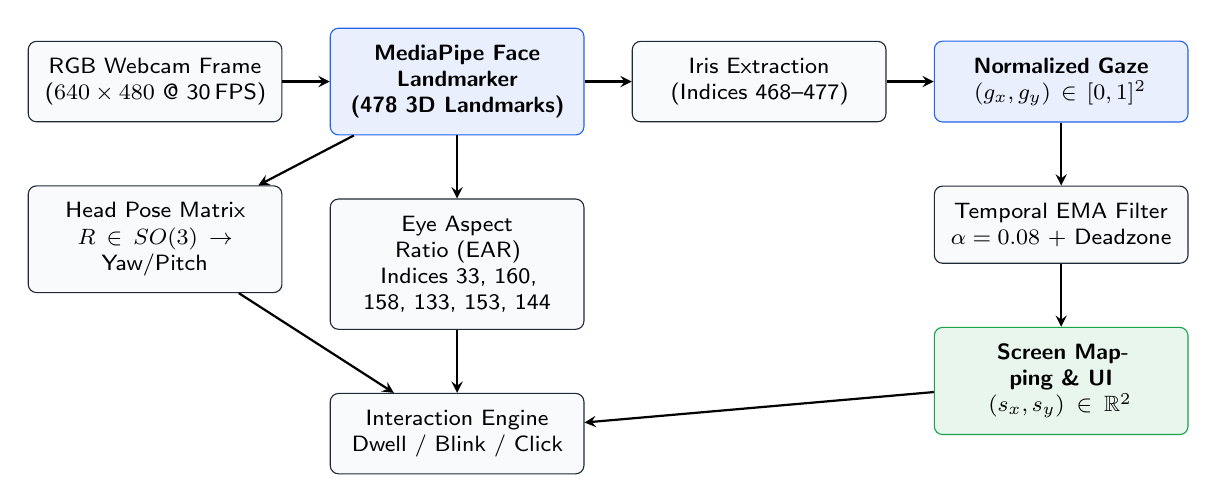
\begin{tikzpicture}[
    node distance=0.8cm and 0.6cm,
    >=stealth,
    every node/.style={transform shape, font=\footnotesize},
    box/.style={rectangle, draw=darkgray, fill=lightbg, rounded corners=3pt, align=center, inner sep=6pt, text width=2.8cm},
    primarybox/.style={rectangle, draw=primaryblue, fill=primaryblue!10, rounded corners=3pt, align=center, inner sep=6pt, text width=2.8cm, font=\footnotesize\bfseries},
    greenbox/.style={rectangle, draw=codegreen, fill=codegreen!10, rounded corners=3pt, align=center, inner sep=6pt, text width=2.8cm, font=\footnotesize\bfseries}
]

    \node (cam) [box] {RGB Webcam Frame\\($640 \times 480$ @ 30\,FPS)};
    \node (mp) [primarybox, right=of cam] {MediaPipe Face Landmarker\\(478 3D Landmarks)};
    \node (iris) [box, right=of mp] {Iris Extraction\\(Indices 468--477)};
    \node (ear) [box, below=of mp] {Eye Aspect Ratio (EAR)\\Indices 33, 160, 158, 133, 153, 144};
    \node (head) [box, below=of cam] {Head Pose Matrix\\$R \in SO(3) \rightarrow$ Yaw/Pitch};
    \node (gaze) [primarybox, right=of iris] {Normalized Gaze\\$(g_x, g_y) \in [0, 1]^2$};
    \node (filter) [box, below=of gaze] {Temporal EMA Filter\\$\alpha=0.08$ + Deadzone};
    \node (screen) [greenbox, below=of filter] {Screen Mapping \& UI\\$(s_x, s_y) \in \mathbb{R}^2$};
    \node (act) [box, below=of ear] {Interaction Engine\\Dwell / Blink / Click};

    \draw[->, thick] (cam) -- (mp);
    \draw[->, thick] (mp) -- (iris);
    \draw[->, thick] (mp) -- (ear);
    \draw[->, thick] (mp) -- (head);
    \draw[->, thick] (iris) -- (gaze);
    \draw[->, thick] (gaze) -- (filter);
    \draw[->, thick] (filter) -- (screen);
    \draw[->, thick] (ear) -- (act);
    \draw[->, thick] (head) -- (act);
    \draw[->, thick] (screen) -- (act);

\end{tikzpicture}
\caption{Real-time sensing and interaction engine architectural pipeline.}
\label{fig:sensing_pipeline}
\end{figure}

% =============================================================================
\section{Mathematical Formulations}
% =============================================================================

\subsection{Eye Aspect Ratio (EAR) \& Blink Detection}
Blink events and eye openness are computed using the scalar ratio of vertical eyelid distances to the horizontal eye width. Given eye landmark points $P_1, P_2, P_3, P_4, P_5, P_6$:
\begin{equation}
\text{EAR} = \frac{\|P_2 - P_6\|_2 + \|P_3 - P_5\|_2}{2 \|P_1 - P_4\|_2 + \epsilon}
\end{equation}
where $\epsilon = 10^{-6}$ prevents numerical division by zero.
A deliberate blink action is classified when:
\begin{equation}
\text{Blink}_{\text{left}} = 
\begin{cases}
1, & \text{if } \text{EAR}_L < \theta_{\text{EAR}} \quad \forall t \in [t_0, t_0 + N_f] \text{ and } (t - t_{\text{last}}) > T_{\text{cool}} \\
0, & \text{otherwise}
\end{cases}
\end{equation}

\subsection{Head Pose Estimation from Transformation Matrix}
From the $4 \times 4$ rigid transformation matrix $M$ computed by the landmark graph, the $3 \times 3$ rotation submatrix $R$ yields Euler angles:
\begin{align}
\text{Yaw}   &= \arctan2\left(R_{1,0}, R_{0,0}\right) \times \frac{180^\circ}{\pi} \\
\text{Pitch} &= \arctan2\left(-R_{2,0}, \sqrt{R_{2,1}^2 + R_{2,2}^2}\right) \times \frac{180^\circ}{\pi}
\end{align}

\subsection{Iris Pupil Gaze Mapping \& Screen Calibration}
Iris center positions $I_x, I_y$ are normalized relative to the inner and outer eye canthi:
\begin{equation}
g_x = \frac{I_x - C_{\text{inner}, x}}{C_{\text{outer}, x} - C_{\text{inner}, x} + \epsilon}
\end{equation}
Using a 4-parameter calibrated bounding box $[x_{\min}, x_{\max}, y_{\min}, y_{\max}]$, screen pixel coordinates $(s_x, s_y)$ are computed by linear min-max normalization:
\begin{equation}
s_x = \text{clip}\left(\frac{g_x - x_{\min}}{x_{\max} - x_{\min}}, 0, 1\right) \times W_{\text{screen}}, \quad
s_y = \text{clip}\left(\frac{g_y - y_{\min}}{y_{\max} - y_{\min}}, 0, 1\right) \times H_{\text{screen}}
\end{equation}

\subsection{Gaze Smoothing \& Jitter Attenuation}
To eliminate ocular micro-tremors and saccadic overshoot without introducing sluggish latency, a first-order Exponential Moving Average (EMA) with deadzone gating is implemented:
\begin{align}
d &= \sqrt{(s_{x, t} - \hat{s}_{x, t-1})^2 + (s_{y, t} - \hat{s}_{y, t-1})^2} \\
\hat{s}_{t} &= 
\begin{cases}
\hat{s}_{t-1}, & \text{if } d \le \delta_{\text{deadzone}} \\
\alpha s_t + (1 - \alpha) \hat{s}_{t-1}, & \text{if } d > \delta_{\text{deadzone}}
\end{cases}
\end{align}

\subsection{Dwell-to-Click State Machine}
Dwell interaction tracks the persistence of gaze coordinates within a spatial radius $\mathcal{R}_{\text{dwell}}$ over elapsed time:
\begin{equation}
P_{\text{dwell}}(t) = \min\left(1.0, \frac{t - t_{\text{anchor}}}{T_{\text{dwell}}}\right)
\end{equation}
When $P_{\text{dwell}}(t) = 1.0$, a system click event is fired and a refractory cooldown $T_{\text{cooldown}}$ is enforced.

% =============================================================================
\section{System Hyperparameters \& Operational Values}
% =============================================================================

This section details all empirical hyperparameters, operational thresholds, temporal windows, and landmark index sets implemented across the sensing, filtering, interaction, and experiment modules.

\begin{table}[H]
\centering
\caption{Complete Specification of System Parameters and Implementation Values.}
\small
\begin{tabularx}{\textwidth}{p{0.28\textwidth} p{0.18\textwidth} p{0.14\textwidth} X}
\toprule
\textbf{Parameter Name} & \textbf{Code Variable} & \textbf{Tuned Value} & \textbf{Functional Role \& Rationale} \\
\midrule
\multicolumn{4}{l}{\textbf{A. Video Acquisition \& Neural Landmark Extraction}} \\
Frame Resolution & \texttt{cap.read()} & $640 \times 480$\,px & Standard webcam resolution balancing speed and detail. \\
Sampling Rate & FPS & 30.0\,FPS & Target acquisition frequency ($\sim 33.3$\,ms/frame). \\
Face Landmark Set & \texttt{face\_landmarks} & 478 points & MediaPipe 3D facial topology. \\
Left Eye Contour & \texttt{LEFT\_EYE} & [33, 160, 158, 133, 153, 144] & Landmark indices used for Left EAR computation. \\
Right Eye Contour & \texttt{RIGHT\_EYE} & [362, 385, 387, 263, 373, 380] & Landmark indices used for Right EAR computation. \\
Left Iris Indices & \texttt{LEFT\_IRIS} & [468, 469, 470, 471, 472] & Iris perimeter and center points for gaze vector. \\
Right Iris Indices & \texttt{RIGHT\_IRIS} & [473, 474, 475, 476, 477] & Contralateral iris landmarks for binocular gaze. \\
\midrule
\multicolumn{4}{l}{\textbf{B. Eye Aspect Ratio (EAR) \& Blink Discrimination}} \\
Left EAR Threshold & \texttt{EAR\_TH\_L} & 0.23 & Below this ratio, left eyelid closure is detected. \\
Right EAR Threshold & \texttt{EAR\_TH\_R} & 0.23 & Below this ratio, right eyelid closure is detected. \\
Blink Frame Persistence & \texttt{CONSEC\_FRAMES} & 4 frames & Minimum frames ($\sim 133$\,ms) to reject micro-blinks. \\
Max Blink Window & \texttt{max\_blink} & 20 frames & $\le 660$\,ms window; longer closures mark drowsiness. \\
Left Click Cooldown & \texttt{CLICK\_COOL} & 0.90\,s & Refractory period preventing unintentional double clicks. \\
\midrule
\multicolumn{4}{l}{\textbf{C. Head Pose \& Calibration Margins}} \\
Yaw Posture Threshold & \texttt{YAW\_TH} & $25.0^\circ$ & Max head turn angle for valid gaze interaction. \\
Pitch Posture Threshold & \texttt{PITCH\_TH} & $20.0^\circ$ & Max vertical tilt angle for valid gaze interaction. \\
Default Gaze Calibration & \texttt{gaze\_calib} & [0.35, 0.65, 0.30, 0.70] & Initial normalized eye-box $[x_{\min}, x_{\max}, y_{\min}, y_{\max}]$. \\
User Profile MSE Cutoff & \texttt{MSE\_CUTOFF} & 0.0035 & Profile matching tolerance for returning users. \\
\midrule
\multicolumn{4}{l}{\textbf{D. Gaze Smoothing \& Dwell Interaction Engine}} \\
EMA Smoothing Factor & \texttt{GAZE\_ALPHA} & 0.08 & Exponential smoothing coefficient ($\alpha \in (0, 1]$). \\
Mouse Deadzone & \texttt{MOUSE\_DEADZONE} & 8\,px & Ignores micro-saccadic tremor below 8 pixels. \\
Mouse Speed Cap & \texttt{MOUSE\_SPEED\_CAP} & 40\,px/frame & Max distance cursor can translate per frame. \\
Dwell Click Hold Time & \texttt{DWELL\_CLICK\_TIME} & 1.50\,s & Required gaze persistence to trigger selection. \\
Dwell Spatial Radius & \texttt{DWELL\_RADIUS\_TH} & 35\,px & Spatial anchor radius bounding the gaze fixation. \\
Dwell Click Cooldown & \texttt{DWELL\_COOLDOWN} & 1.80\,s & Cooldown following dwell selection before next dwell. \\
\midrule
\multicolumn{4}{l}{\textbf{E. Experimental Timing \& Stimulus Progression}} \\
Overt Memorize Window & \texttt{MEMORIZE\_SECS} & 15.0\,s & Countdown duration for overt prompt memorization. \\
Instructions Countdown & \texttt{secs=5} & 5.0\,s & Auto-advance timer on instruction screen. \\
Fixation Cross Duration & \texttt{secs=5} & 5.0\,s & Center gaze fixation interval before each trial. \\
Inter-Trial Rest Break & \texttt{REST\_DURATION} & 30.0\,s & Pause duration with audio TTS guidance. \\
Trial Count per Session & \texttt{TRIALS\_PER\_SESSION} & 8 trials & 5 canonical words + 3 pangram phrases. \\
\bottomrule
\end{tabularx}
\end{table}

% =============================================================================
\section{Text Entry Evaluation Metrics \& Formulation}
% =============================================================================

Experimental text composition is evaluated through the following standardized HCI and typing metrics:

\begin{table}[H]
\centering
\caption{Mathematical Definitions of Experimental Typing Metrics.}
\small
\begin{tabularx}{\textwidth}{p{0.25\textwidth} p{0.35\textwidth} X}
\toprule
\textbf{Metric} & \textbf{Mathematical Formula} & \textbf{Description} \\
\midrule
\textbf{Words Per Minute (WPM)} & $\text{WPM} = \frac{|T| - 1}{S} \times 60 \times \frac{1}{5}$ & Net composition speed normalized to 5-character word equivalents over duration $S$ seconds. \\
\textbf{Keystrokes Per Char (KSPC)} & $\text{KSPC} = \frac{|K|}{|T|}$ & Ratio of total registered key actions $|K|$ to final produced transcript length $|T|$. \\
\textbf{Character Error Rate (CER)} & $\text{CER} = \frac{\text{Levenshtein}(T, I)}{\max(|T|, |I|)} \times 100\%$ & Minimum edit distance between typed string $T$ and stimulus prompt $I$. \\
\textbf{Inter-Key Interval (IKI)} & $\text{IKI}_i = t_{k_i} - t_{k_{i-1}}$ & Temporal gap between consecutive character selections. \\
\textbf{Cognitive Latency (CLPI)} & $\text{CLPI} = t_{k_1} - t_{\text{stimulus\_onset}}$ & Preparation and visual search interval before the first key press. \\
\bottomrule
\end{tabularx}
\end{table}

% =============================================================================
\section{Experimental Paradigms \& Standardized Stimuli}
% =============================================================================

The evaluation platform supports two distinct cognitive-motor experimental methods:
\begin{enumerate}
    \item \textbf{Overt Method}: Stimulus is shown during a 15-second memorization window with a progress countdown. The prompt is hidden upon entering the typing phase, testing recall, spatial gaze orientation, and working memory.
    \item \textbf{Covert Method}: Stimulus remains permanently visible directly above the typing input box, isolating pure gaze-motor speed and perceptual targeting.
\end{enumerate}

\subsection{Standardized Canonical Stimulus Set (8 Trials Total)}
To ensure rigorous cross-participant consistency, stimuli are drawn from a deterministic canonical pool:
\begin{itemize}
    \item \textbf{Words (5 items)}: \texttt{help}, \texttt{food}, \texttt{table}, \texttt{chair}, \texttt{smile}.
    \item \textbf{Phrases (3 pangrams)}:
    \begin{enumerate}
        \item \emph{``The quick brown fox jumps over the lazy dog.''} (43 characters)
        \item \emph{``Pack my box with five dozen liquor jugs.''} (39 characters)
        \item \emph{``Sphinx of black quartz, judge my vow.''} (37 characters)
    \end{enumerate}
\end{itemize}

\subsection{Interleaved Trial Progression Sequence}
\begin{equation}
\text{Trial Sequence} = \underbrace{W_1 \rightarrow W_2}_{\text{Words}} \rightarrow \underbrace{P_1}_{\text{Phrase}} \rightarrow \underbrace{W_3 \rightarrow W_4}_{\text{Words}} \rightarrow \underbrace{P_2}_{\text{Phrase}} \rightarrow \underbrace{W_5}_{\text{Word}} \rightarrow \underbrace{P_3}_{\text{Phrase}}
\end{equation}

Between trials, an automated 30-second resting break screen suspends camera capture, announces tracker state via text-to-speech audio, and resets cursor position to screen center $(W/2, H/2)$ upon resumption.

% =============================================================================
\section{Future Work \& Proposed Development}
% =============================================================================

The current system provides a foundation for real-time eye tracking, gaze-based typing, attention monitoring, gaze cursor control, heatmap generation, and automated experimental reporting. The next phase of development will extend the system from a primarily application-level eye-tracking interface into a comprehensive hands-free accessibility and communication platform.

% -----------------------------------------------------------------------------
\subsection{Enhanced Virtual Keyboard and Word Navigation}
% -----------------------------------------------------------------------------

The existing gaze-based virtual keyboard will be enhanced to provide more efficient text editing and navigation. In addition to character-level typing, dedicated navigation controls will be introduced for moving between words.

The proposed keyboard controls include:
\begin{itemize}
    \item \textbf{Word Left}: Moves the text cursor one word toward the left.
    \item \textbf{Word Right}: Moves the text cursor one word toward the right.
    \item \textbf{Backspace}: Deletes the character immediately preceding the cursor.
    \item \textbf{Delete Word}: Removes the currently selected or preceding word.
    \item \textbf{Clear}: Clears the current text input.
    \item \textbf{Space}: Inserts a space between words.
    \item \textbf{Enter}: Confirms or submits the current input.
\end{itemize}

These controls reduce the need for character-by-character correction and make gaze-based text composition faster and more practical for users with severe motor impairments.

% -----------------------------------------------------------------------------
\subsection{Family Communication and Phrase-Based Messaging}
% -----------------------------------------------------------------------------

A dedicated communication module allows users to communicate directly with selected family members or caregivers. The workflow is modeled as:
\begin{equation}
\text{Gaze Selection} \rightarrow \text{Contact Selection} \rightarrow \text{Phrase Selection} \rightarrow \text{Message Composition} \rightarrow \text{Message Transmission}
\end{equation}
High-priority phrases such as \emph{``I need help''}, \emph{``Please come here''}, and \emph{``I am thirsty''} are rendered as high-contrast gaze targets with integrated SOS SMS/WhatsApp dispatch via background API workers.

% -----------------------------------------------------------------------------
\subsection{Full Computer and Windows Accessibility Control}
% -----------------------------------------------------------------------------

Extending the system beyond the local GUI window into a system-wide OS accessibility layer enables hands-free operation across arbitrary third-party software. The command set includes:
\begin{itemize}
    \item \textbf{Mouse Movement}: Continuous gaze-driven cursor translation.
    \item \textbf{Discrete Actions}: Single Click, Double Click, Right Click, Click \& Drag.
    \item \textbf{Document Navigation}: Smooth Scroll Up/Down, Page Up/Down.
    \item \textbf{Window Management}: Application Switching, Minimize, Maximize, Close.
\end{itemize}

% -----------------------------------------------------------------------------
\subsection{Assistive Health and Pain Communication}
% -----------------------------------------------------------------------------

To facilitate clinical and home-care interaction, a structured health assessment matrix allows users to communicate discomfort:
\begin{equation}
\text{Pain Level (1--10)} + \text{Body Region} + \text{Pain Characteristic} + \text{Custom Note} \rightarrow \text{Caregiver Alert}
\end{equation}

% -----------------------------------------------------------------------------
\subsection{Unified Accessibility Architecture}
% -----------------------------------------------------------------------------

\begin{figure}[H]
\centering
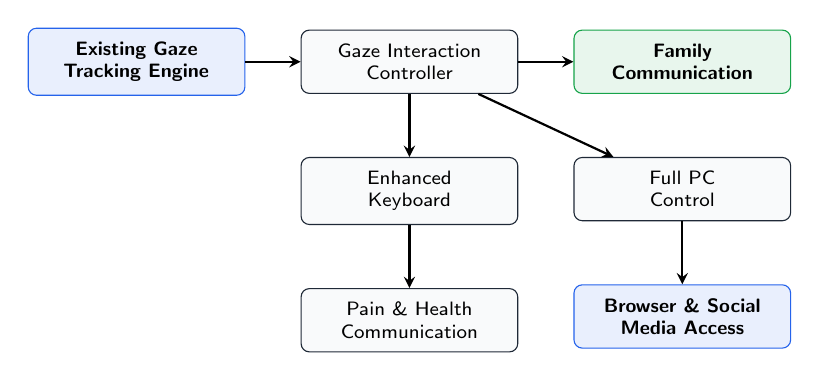
\begin{tikzpicture}[
    node distance=0.8cm and 0.7cm,
    >=stealth,
    every node/.style={transform shape, font=\scriptsize},
    archnode/.style={rectangle, draw=darkgray, fill=lightbg, rounded corners=3pt, align=center, inner sep=5pt, text width=2.4cm},
    bluenode/.style={rectangle, draw=primaryblue, fill=primaryblue!10, rounded corners=3pt, align=center, inner sep=5pt, text width=2.4cm, font=\scriptsize\bfseries},
    greennode/.style={rectangle, draw=codegreen, fill=codegreen!10, rounded corners=3pt, align=center, inner sep=5pt, text width=2.4cm, font=\scriptsize\bfseries}
]

    \node (gaze) [bluenode] {Existing Gaze\\Tracking Engine};
    \node (controller) [archnode, right=of gaze] {Gaze Interaction\\Controller};
    \node (keyboard) [archnode, below=of controller] {Enhanced\\Keyboard};
    \node (comm) [greennode, right=of controller] {Family\\Communication};
    \node (pc) [archnode, below=of comm] {Full PC\\Control};
    \node (health) [archnode, below=of keyboard] {Pain \& Health\\Communication};
    \node (web) [bluenode, below=of pc] {Browser \& Social\\Media Access};

    \draw[->, thick] (gaze) -- (controller);
    \draw[->, thick] (controller) -- (keyboard);
    \draw[->, thick] (controller) -- (comm);
    \draw[->, thick] (controller) -- (pc);
    \draw[->, thick] (keyboard) -- (health);
    \draw[->, thick] (pc) -- (web);

\end{tikzpicture}
\caption{Proposed future architecture for the unified gaze-based accessibility platform.}
\label{fig:future_unified_arch}
\end{figure}

% -----------------------------------------------------------------------------
\subsection{Development Roadmap}
% -----------------------------------------------------------------------------

\begin{table}[H]
\centering
\caption{Incremental Development Roadmap.}
\small
\begin{tabularx}{\textwidth}{p{0.14\textwidth} p{0.26\textwidth} X}
\toprule
\textbf{Phase} & \textbf{Feature Domain} & \textbf{Primary Technical Objective} \\
\midrule
Phase 1 & Enhanced Virtual Keyboard & Word-level navigation (Word Left/Right), word deletion, and cluster optimizations. \\
Phase 2 & Caregiver Communication & Emergency SOS dispatch, contact lists, and canned phrase selection. \\
Phase 3 & OS Desktop Accessibility & Global mouse hooks, double-click/right-click dwell modals, and scrolling overlays. \\
Phase 4 & Assistive Health & 1--10 visual pain scale, body anatomical map selector, and caregiver logs. \\
Phase 5 & Web \& Social Media & Gaze-assisted browser navigation, form interaction, and social chat integration. \\
Phase 6 & Unified Platform & Consolidated monolithic runtime with automatic calibration profile management. \\
\bottomrule
\end{tabularx}
\end{table}

% =============================================================================
\section{Conclusion}
% =============================================================================

The described eye-tracking and AAC platform demonstrates the feasibility of combining computer vision landmark graphs with human-computer interaction heuristics on uncalibrated consumer webcams. The integration of robust EAR blink discrimination, EMA deadzone smoothing, structured 8-trial experimental evaluation, and future-oriented OS control provides a comprehensive framework for both experimental HCI research and real-world assistive communication.

\end{document}
